\documentclass[12pt]{article}
\usepackage[margin=1in]{geometry}
\usepackage{fancyvrb}
\usepackage{multicol}
\usepackage{hyperref}
\usepackage{amsmath}

\usepackage[listings]{tcolorbox}

\definecolor{codegreen}{rgb}{0,0.6,0}
\definecolor{codegray}{rgb}{0.5,0.5,0.5}
\definecolor{codepurple}{rgb}{0.58,0,0.82}
\definecolor{backcolour}{rgb}{0.95,0.95,0.92}

\lstdefinestyle{mystyle}{
    language=Python,
    backgroundcolor=\color{backcolour},   
    commentstyle=\color{codegreen},
    keywordstyle=\color{magenta},
    numberstyle=\tiny\color{codegray},
    stringstyle=\color{codepurple},
    basicstyle=\ttfamily\footnotesize,
    breakatwhitespace=false,         
    breaklines=true,                 
    captionpos=b,                    
    keepspaces=true,                 
    numbers=left,                    
    numbersep=5pt,                  
    showspaces=false,                
    showstringspaces=false,
    showtabs=false,                  
    tabsize=2,
    escapechar=|,
    frame=single
}

\lstset{style=mystyle}
\begin{document}
\sloppy
\centerline{\Large CSCI 111, Lab 7}
\centerline{\large Image Processing}

\begin{description}
\item[Due date:] Midnight, Tuesday, November 1, on Canvas.
No late work accepted.  

\item[File names:]  Names of files, functions, and variables, 
when specified,
must be EXACTLY as specified.  This includes simple mistakes such
as capitalization.

\item[Individual work:]  All work must be your own.  Do not share
code with anyone other than the instructor and teaching assistants.
This includes looking over shoulders at screens with the code open.
You may discuss ideas, algorithms, approaches, {\em etc.} with
other students but NEVER actual code.

\item[Image processing:]  Two dimensional color images are stored
on computers in a two dimensional array of colors.  A color is a 
triple of red, green, and blue integer values, each in the range [0,255].
Thus, red is (255,0,0), green is (0, 255, 0), blue is (0, 0, 255)
and yellow is (255, 255, 0).  Black is (0,0,0) and white is (255, 255, 255).

The PIL module provides functions for loading and storing images
on disk in many formats.  It also allows you to get  and
set the color for any pixel.  Demonstrations of how to use 
some of its routines are provided in my demonstration files
in the lab folder.

{\bf Important:} do not use any PIL routines except the ones
deonstrated in my code.  PIL is a very powerful image processing
library and can easily do many of the tasks I've set for you below.
But you have to do them only with getpixel and setpixel.  All the
rest is done in Python without PIL routines.

Because we're going to process images with mathematical functions,
it will be much easier to deal with colors as a triple of 
floating point numbers between 0 and 1.  My \lstinline{getpixel}
and \lstinline{setpixel} functions will handle this conversion
for you.  All computation with colors is done on floats in [0,1], not
ints in [0,255]

\item[Provided code:] I have provided three modules:
\begin{description}
\item[\tt pixel.py]  Simple utilities for getting/setting
pixels and converting from ints in [0,255] to/from floats
in [0,1]
\item[\tt separation.py] Simple image processing that
just extracts the red, green, and blue components of an image.
\item[\tt demo.py] A demo program using \lstinline{tkinter}
that will open an image file and run several image processing
algorithms on the image, and show the results in a new window.

Simply comment out the parts that aren't finished until you 
finish them!
\end{description}

\item[Extract colors:]  One of the things you can do with an image
is just erase two of the three colors.  I've done this in
the \lstinline{separation} module, so you can see the effect.

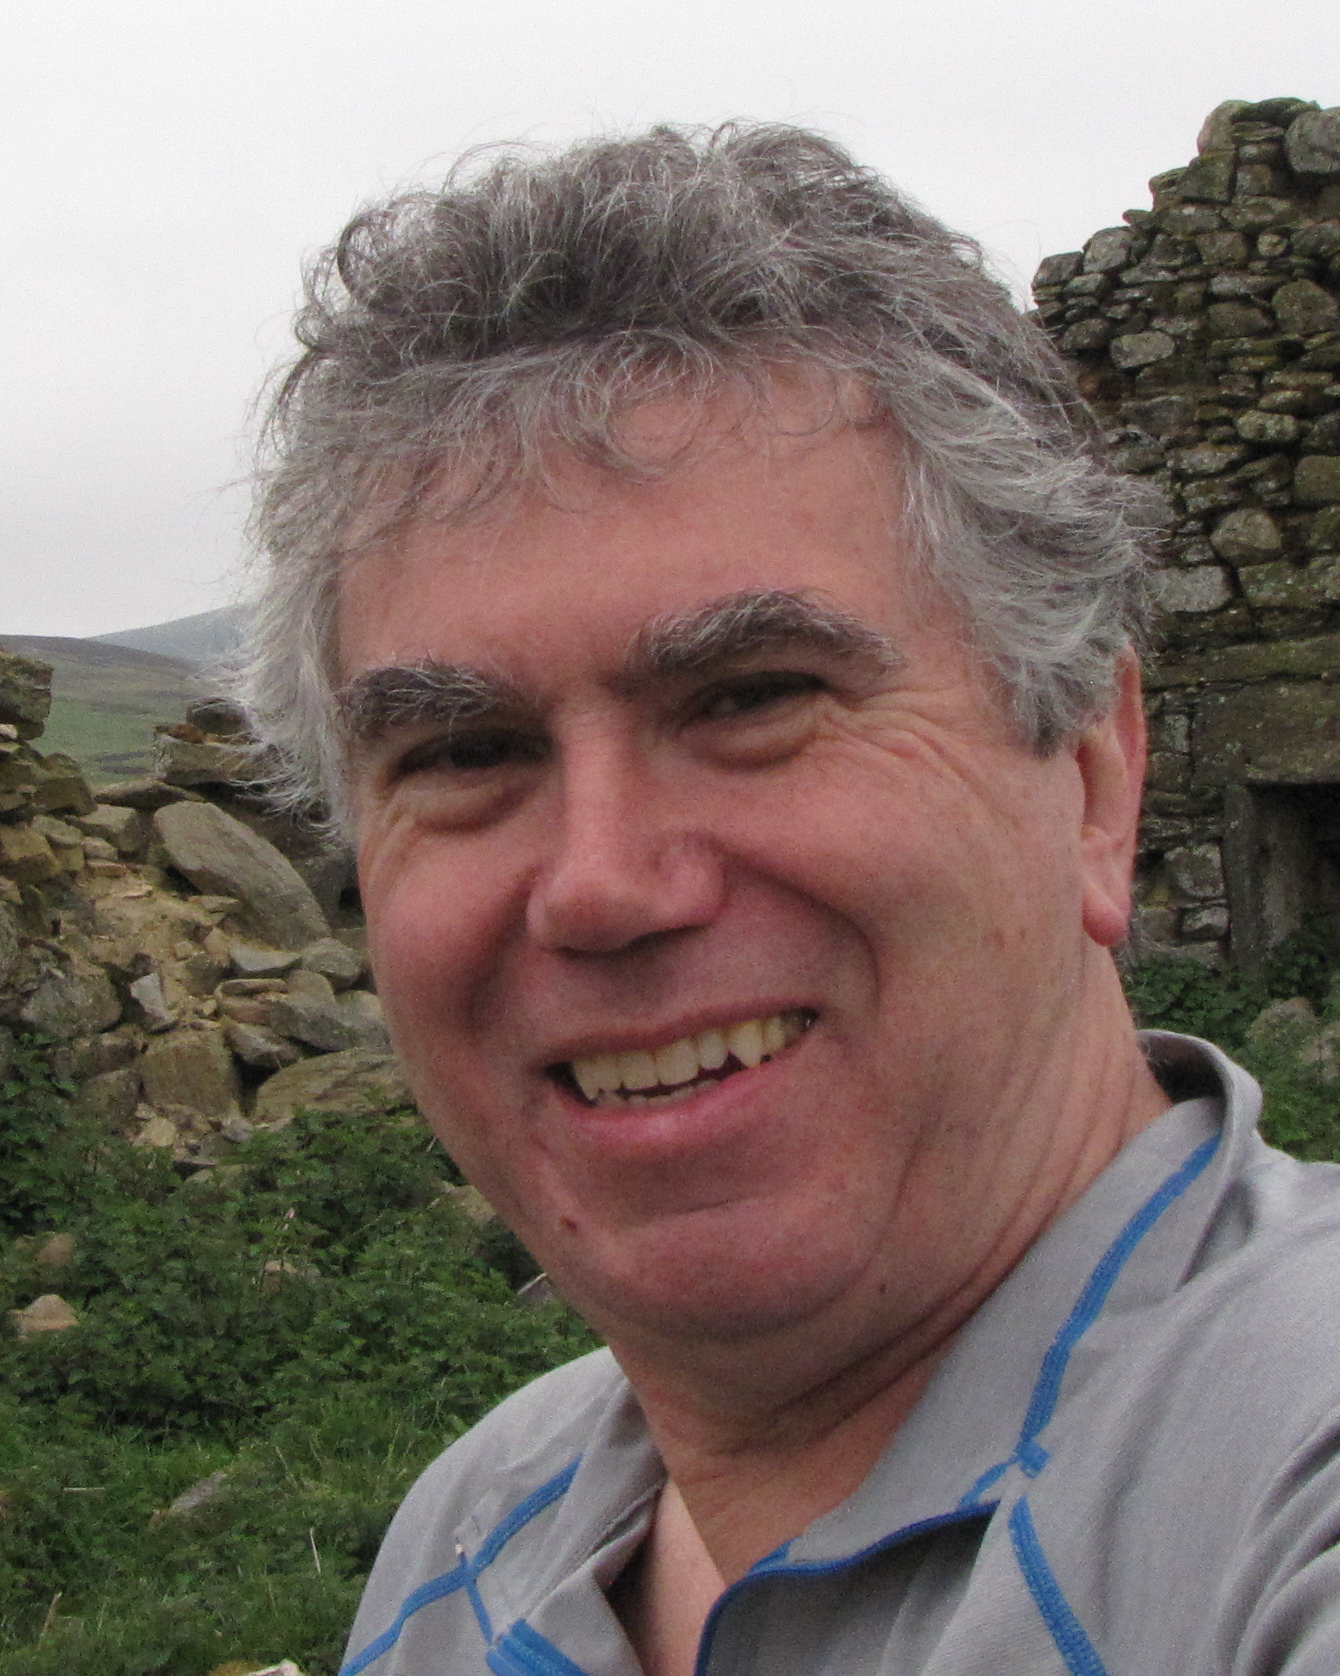
\includegraphics[scale=0.18]{geoffinscotland.png}
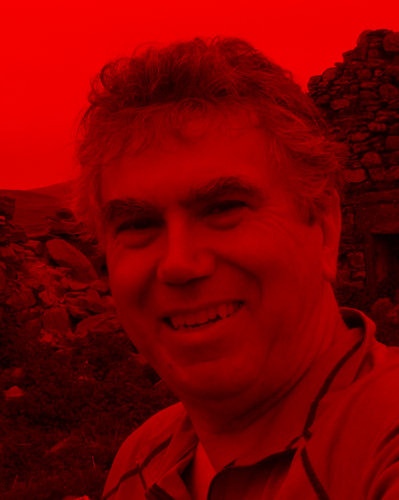
\includegraphics[scale=0.25]{red.png}
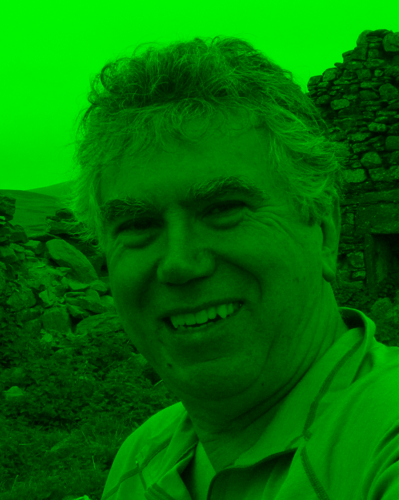
\includegraphics[scale=0.25]{green.png}
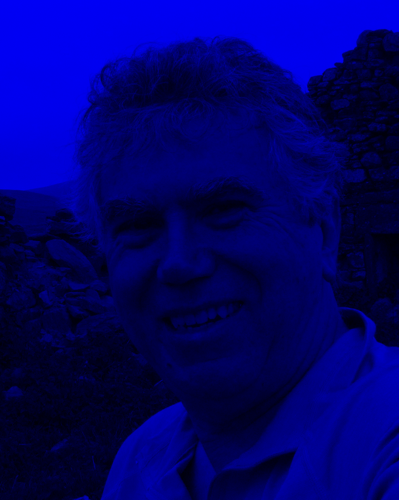
\includegraphics[scale=0.25]{blue.png}

\item[Grayscale:]  Turning a color image into grayscale is just
a matter of adding up all the colors to get a total {\bf luminance}
value for the pixel.  Because our eyes are more sensitive to 
green and red than blue, the sum should be weighted as follows:
\[
gray=0.299red+0.587green+0.114blue
\]
Rather than just taking 1/3 each.
You can try both and see which one you like better.

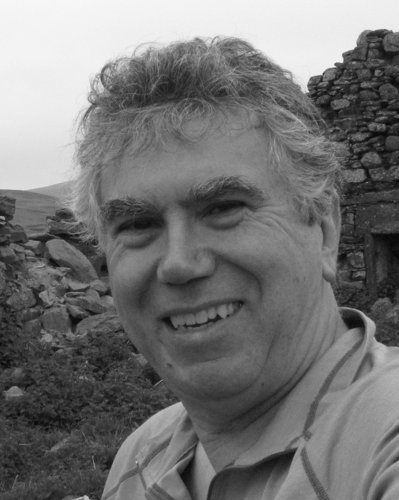
\includegraphics[scale=0.25]{gray.png}


\item[Posterize:] Posterizing an image means turning bands
of the same luminance into different colors.  For example
I used black for luminance less than 25\%,
red for 25\% to 50\%, magenta for 50\% to 75\%,
and white for 75\% to 100\%.

Play around with different color bands at different
percentages until you get one you like.

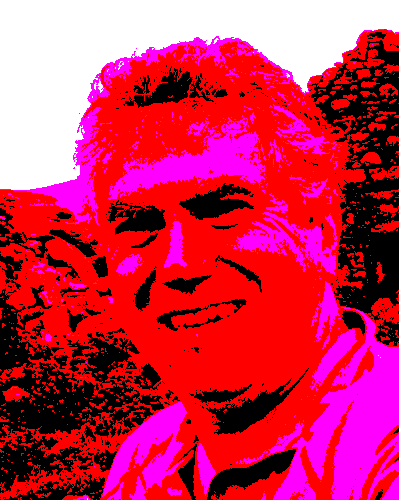
\includegraphics[scale=0.25]{poster.png}


\item[Edge detection:] Edge detection is a difficult and
ongoing field of research.  However, a simple algorithm
works fairly well.  Compute the following quantities
for a pixel at $(x,y)$, where $L(x,y)$ is the luminance
at $(x,y)$:
\begin{align*}
L_x(x,y) &= \frac{L(x,y+1) - L(x,y-1)}{2}\\
L_y(x,y) &= \frac{L(x+1,y) - L(x-1,y)}{2}\\
|\nabla L(x,y)| &= \sqrt{L_x(x,y)^2 + L_y(x,y)^2}
\end{align*}
The quantity $|\nabla L(x,y)|$ is the magnitude of the gradient.
The larger this value is, the more rapidly the luminance
of the image is changing.

If we color only the values of large gradient, we should be
coloring the lines.   This is just posterizing with
white below a threshold and black above.

You may have to tweak the threshold a bit
to get the best lines.  Try looking at the gradient
value without thresholding to see if you're on the right 
track. Remember:  this is a difficult problem.
You're not going to get perfect lines.  :(

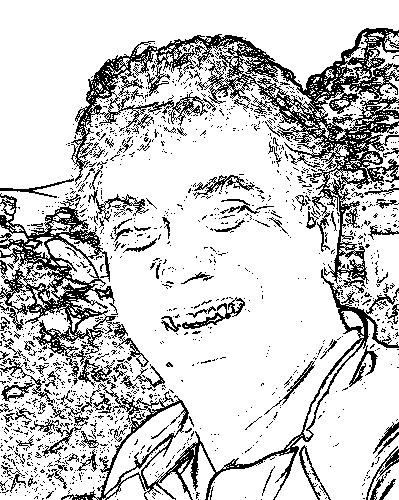
\includegraphics[scale=0.25]{edge.png}


\item[Hand in:] Include my images and code in your \lstinline{lab07}
folder, along with your own implementation of the module
\lstinline{imageprocessing.py} including routines
\begin{itemize}
\item \lstinline{grayscale}
\item \lstinline{posterize}  (your colors don't have to match mine)
\item \lstinline{edge_detect}
\end{itemize}
Also include an image of your own! I'd prefer your face, but the
choice is yours.

Make sure your module works with my demo program!  You should
not have to change anything in \lstinline{demo.py}

\item[Bonus:]  One bonus lab point!  Do {\bf sepia}
as found here 

\url{https://dyclassroom.com/image-processing-project/how-to-convert-a-color-image-into-sepia-image}

Remember that our colors have been converted from 
integers in [0,255] to floats in [0,1].  Do your 
processing with the floats.


\end{description}
\end{document}
